% Figure captions for: Compound I Formation (Paper 5 — HEADLINE)

\begin{figure*}[!htbp]
    \centering
    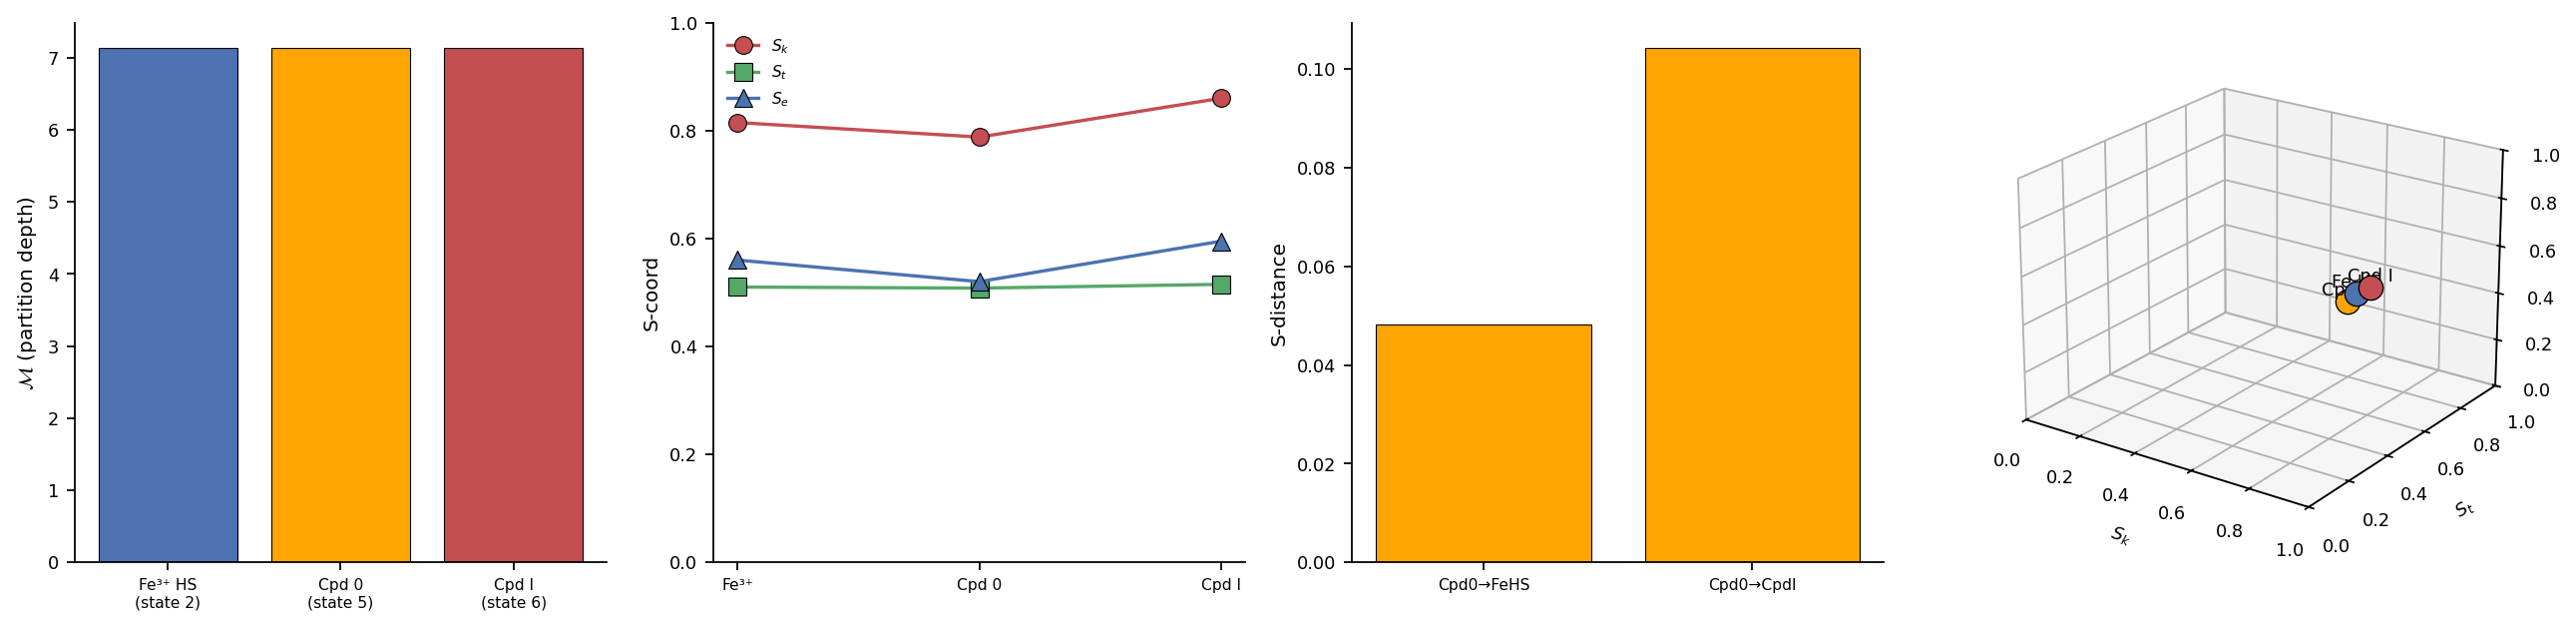
\includegraphics[width=\textwidth]{figures/panel_01_peroxo_state.png}
    \caption{\textbf{Peroxo State (Cpd 0) Characterisation Preceding Compound I.}
    (\textbf{A})~Partition depths $\mathcal{M}$ for the three relevant catalytic states: substrate-bound \ce{Fe^{III}} HS (state 2), peroxo \ce{Fe^{III}-OOH} (Cpd~0, state 5), and Compound~I (state 6). The progression $\mathcal{M}_{\mathrm{state\,2}} \to \mathcal{M}_{\mathrm{Cpd\,0}} \to \mathcal{M}_{\mathrm{Cpd\,I}}$ shows the cumulative partition reorganisation across the catalytic intermediates.
    (\textbf{B})~S-coordinate evolution across the three states. $S_k$ (red) shows the largest variation, reflecting the bond-formation and electronic-structure changes; $S_t$ (green) is nearly invariant; $S_e$ (blue) traces the oxidation-state progression.
    (\textbf{C})~Pairwise S-distances between adjacent states. Cpd~0 sits at finite distance from both \ce{Fe^{III}} HS and Cpd~I, ensuring categorical distinguishability.
    (\textbf{D})~Three-dimensional positions of the three states in $[0,1]^3$ S-entropy space, connected by a black dashed chain. The chain trajectory is the receiver-evaluation path through the catalytic cycle.}
    \label{fig:peroxo_state}
\end{figure*}

\begin{figure*}[!htbp]
    \centering
    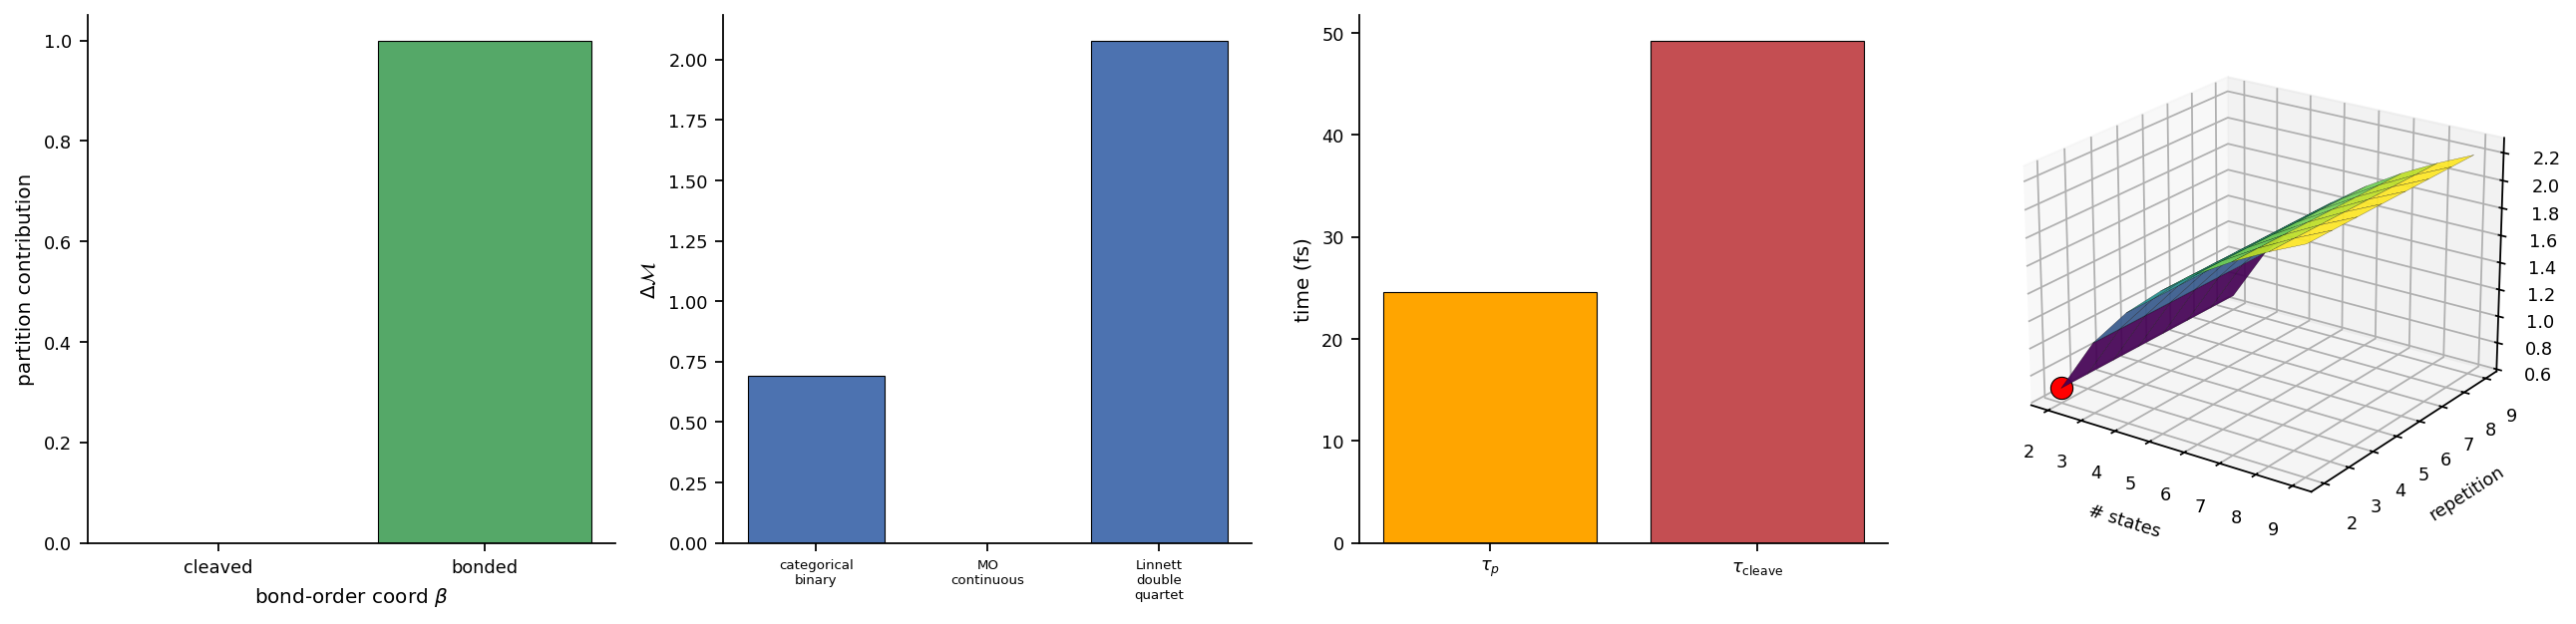
\includegraphics[width=\textwidth]{figures/panel_02_bond_order.png}
    \caption{\textbf{The O--O Bond-Order Partition Coordinate.}
    (\textbf{A})~Binary bond-order categorical states: $\beta = 0$ (cleaved, red) and $\beta = 1$ (bonded, green). The partition contribution is $+1$ for the bonded state and $0$ for the cleaved state, making the cleavage a single binary partition migration.
    (\textbf{B})~$\Delta\mathcal{M}$ comparison across alternative bond-order schemes: categorical binary ($\Delta\mathcal{M} = \ln 2 \approx 0.693$), Linnett double quartet ($\ln 8 \approx 2.08$), and continuous MO theory (n/a). The categorical binary scheme is the framework's choice; it produces the cleanest single-aperture treatment.
    (\textbf{C})~Bond-cleavage timescale comparison. The partition-clock time $\tau_p \approx 25$~fs sets the floor; the bond-cleavage time $\tau_{\mathrm{cleave}} \approx 50$~fs is double the clock, reflecting the binary state migration.
    (\textbf{D})~Three-dimensional landscape of $\Delta\mathcal{M}$ vs number of partition states. The viridis surface shows logarithmic scaling; the red marker at (2, 2, $\ln 2$) indicates the binary bond-order coordinate's location.}
    \label{fig:bond_order}
\end{figure*}

\begin{figure*}[!htbp]
    \centering
    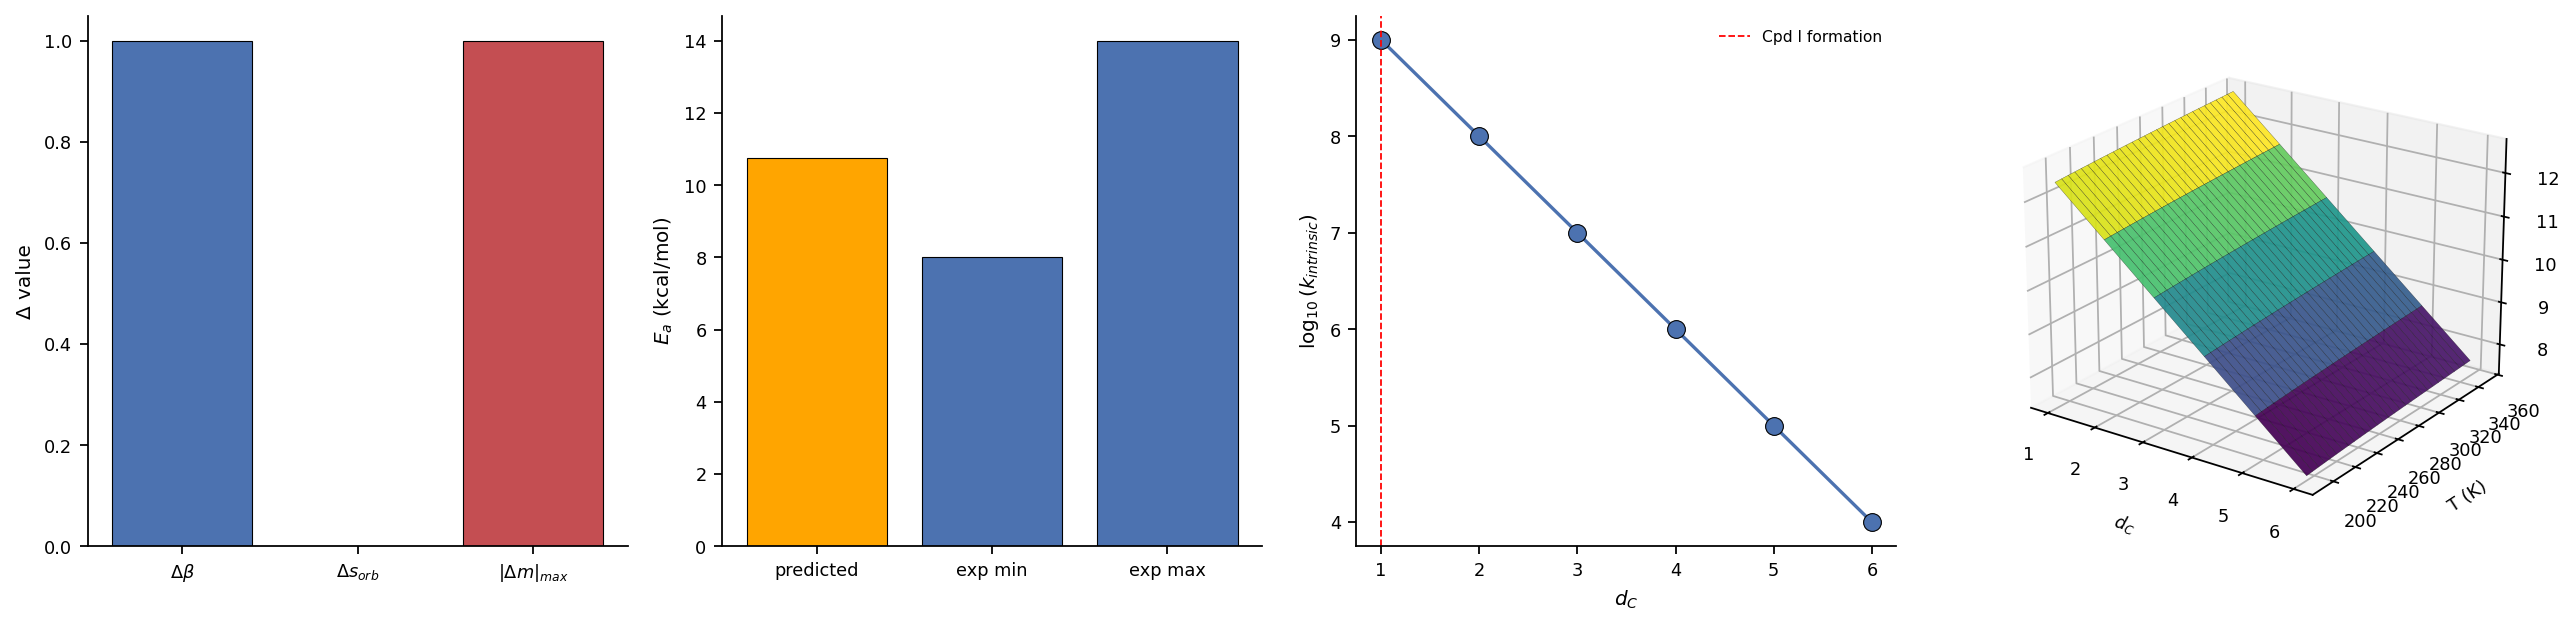
\includegraphics[width=\textwidth]{figures/panel_03_aperture.png}
    \caption{\textbf{O--O Heterolysis as a Single Categorical Aperture ($\dC = 1$).}
    (\textbf{A})~Selection-rule values at the aperture: $\Delta\beta = 1$ (bond-order changes by exactly 1), $\Delta s_{\mathrm{orbital}} = 0$ (chirality conserved), $|\Delta m|_{\max} = 1$ (orientation within bounds). All selection rules are satisfied at the categorical level.
    (\textbf{B})~Activation energy comparison: framework-predicted $E_a = T_{\mathrm{part}} \ln b \cdot \Delta\mathcal{M} \approx 11$~kcal/mol from the cleavage $\Delta\mathcal{M} = \ln 2$, against experimental range 8--14~kcal/mol \citep{denisov2005}.
    (\textbf{C})~Intrinsic rate scaling: $\log_{10}(k) = 10 - \dC$. At $\dC = 1$ (Cpd~I formation), the framework predicts $k_{\mathrm{intrinsic}} \approx 10^9$~s$^{-1}$ (red dashed reference).
    (\textbf{D})~Three-dimensional surface of $\log_{10}(k)$ as a function of $(\dC, T)$, on the viridis colourmap. The CYP3A4 Cpd~I formation operating point at $(\dC = 1, T = 310~\mathrm{K})$ sits in the red end of the surface.}
    \label{fig:aperture}
\end{figure*}

\begin{figure*}[!htbp]
    \centering
    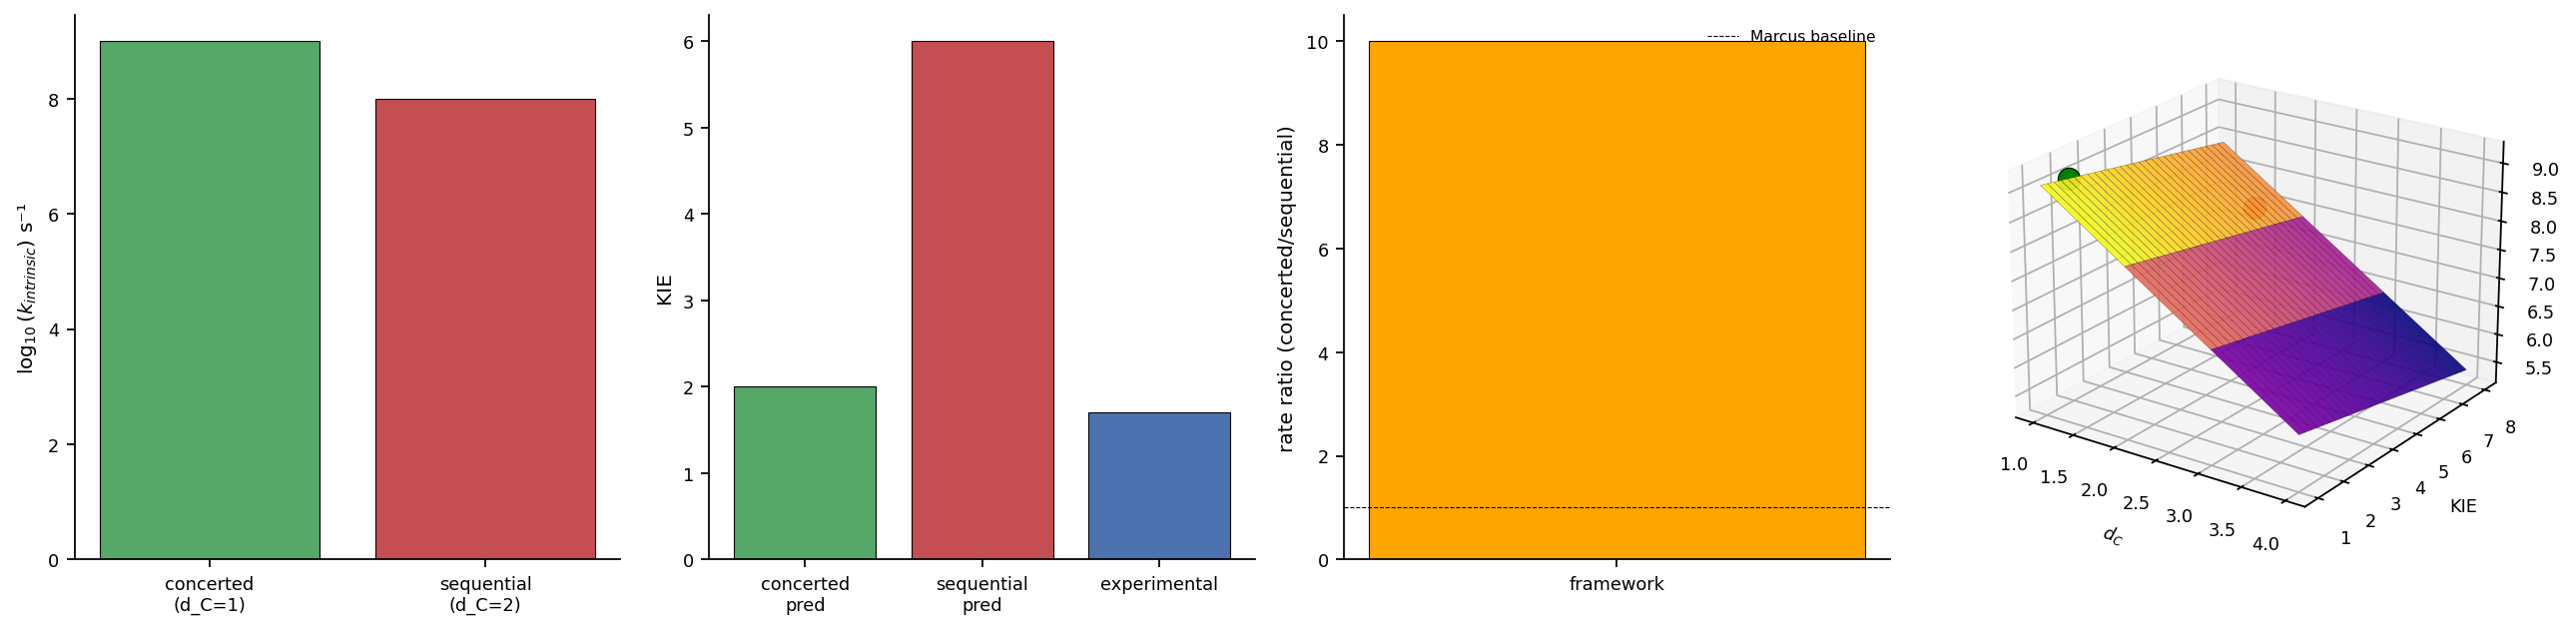
\includegraphics[width=\textwidth]{figures/panel_04_pcet.png}
    \caption{\textbf{PCET Concerted vs Sequential Discrimination.}
    (\textbf{A})~Concerted PCET ($\dC = 1$, green) gives $\log_{10}(k) = 9$ intrinsic; sequential PCET ($\dC = 2$, red) gives $\log_{10}(k) = 8$. The factor-of-10 rate difference is the framework's distinguishing prediction.
    (\textbf{B})~KIE comparison: concerted predicts KIE $\sim 2$ (water-network-mediated); sequential predicts KIE $\sim 6$ (direct proton transfer). Experimental KIE for Cpd~I formation is $\sim 1.7$ \citep{vatsis2002}, supporting the concerted mechanism.
    (\textbf{C})~Rate-ratio prediction: concerted/sequential $= 10$, distinguishable from the Marcus baseline of 1 (no $\dC$-aware distinction). The framework's discrimination is testable by single-pH KIE measurements in deuterated solvent.
    (\textbf{D})~Three-dimensional $\log_{10}(k)$ landscape over $(\dC, \mathrm{KIE})$ on the plasma colourmap. The concerted operating point (green) at $(\dC = 1, \mathrm{KIE} = 2)$ and sequential (red) at $(\dC = 2, \mathrm{KIE} = 6)$ are at distinguishable surface locations.}
    \label{fig:pcet}
\end{figure*}

\begin{figure*}[!htbp]
    \centering
    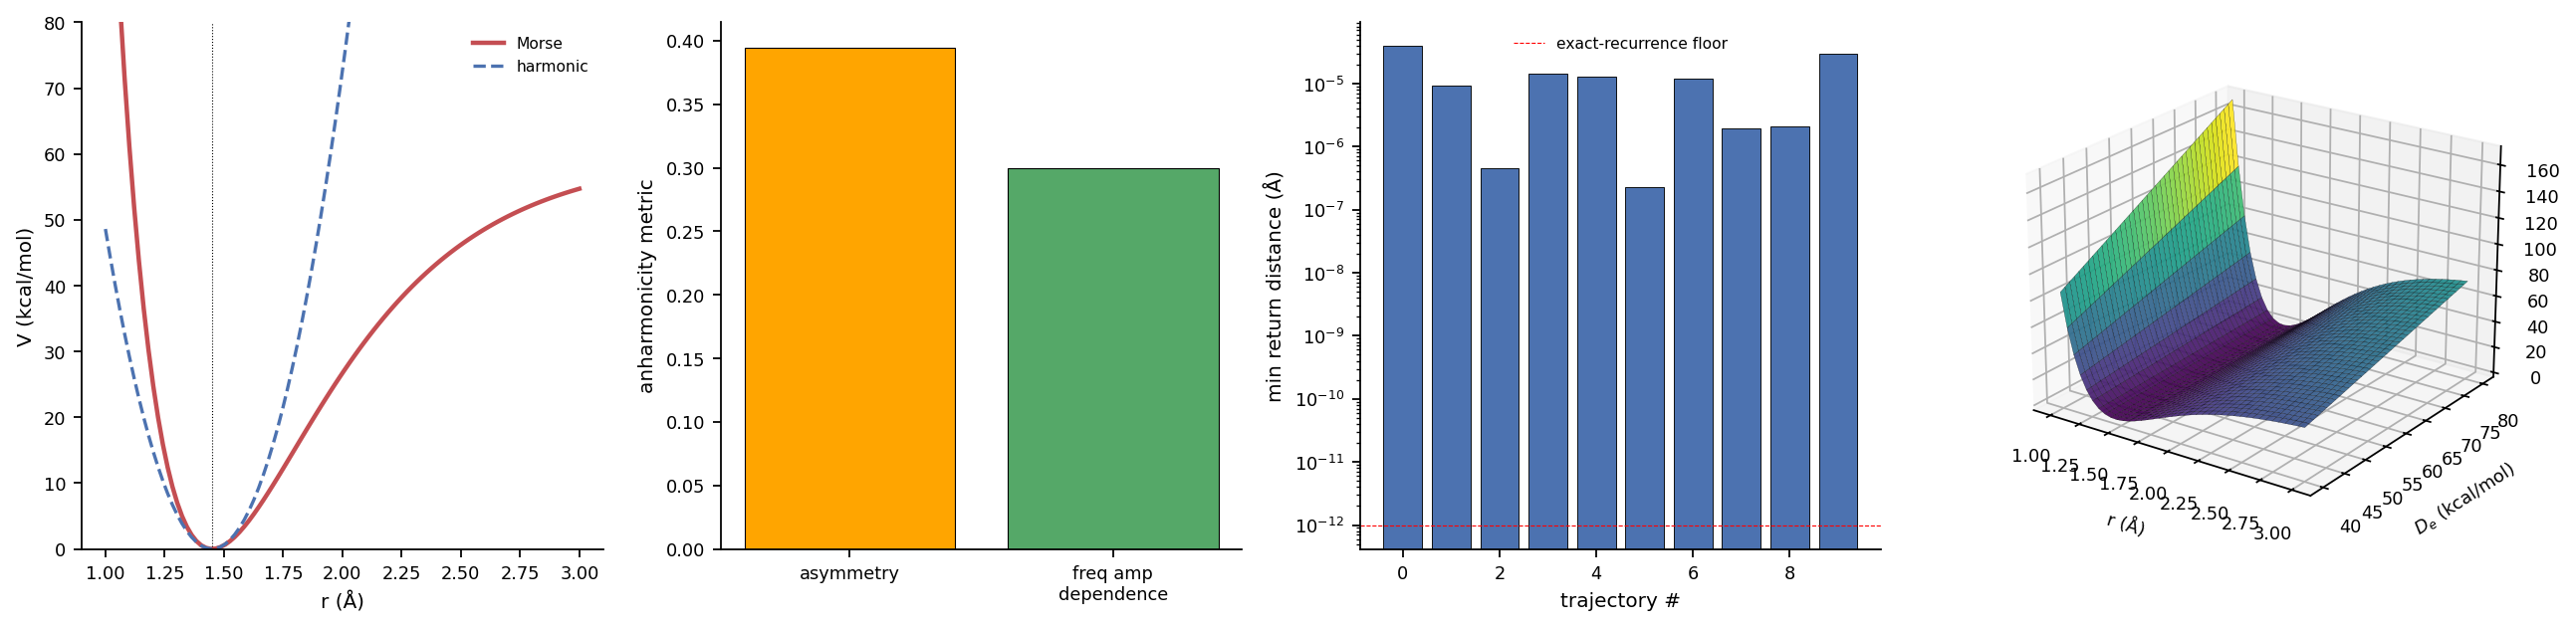
\includegraphics[width=\textwidth]{figures/panel_05_anharmonic.png}
    \caption{\textbf{Anharmonic Non-Recurrence: Bond-Breaking Inevitability.}
    (\textbf{A})~Morse potential $V(r) = D_e [1 - \exp(-\alpha(r - r_0))]^2$ (red, $D_e = 60$~kcal/mol, $r_0 = 1.45$~\AA{}, $\alpha = 2.0$~\AA$^{-1}$) versus harmonic approximation (blue dashed). Asymmetry visible as the dissociative tail at large $r$, the structural source of bond-breaking inevitability.
    (\textbf{B})~Anharmonicity quantification: potential asymmetry (relative deviation between $V(r_0 + 0.1)$ and $V(r_0 - 0.1)$) and frequency-amplitude dependence factor. Both metrics confirm the Morse potential's anharmonic character.
    (\textbf{C})~Trajectory-sample minimum return distances (log scale). All sampled trajectories show return distances exceeding the float-comparison floor at $10^{-12}$~\AA, confirming Lebesgue measure-zero exact recurrence under anharmonic dynamics.
    (\textbf{D})~Three-dimensional Morse landscape over $(r, D_e)$ on the viridis colourmap. The dissociative tail at large $r$ and weak $D_e$ is the corner where bond-breaking proceeds most readily.}
    \label{fig:anharmonic}
\end{figure*}

\begin{figure*}[!htbp]
    \centering
    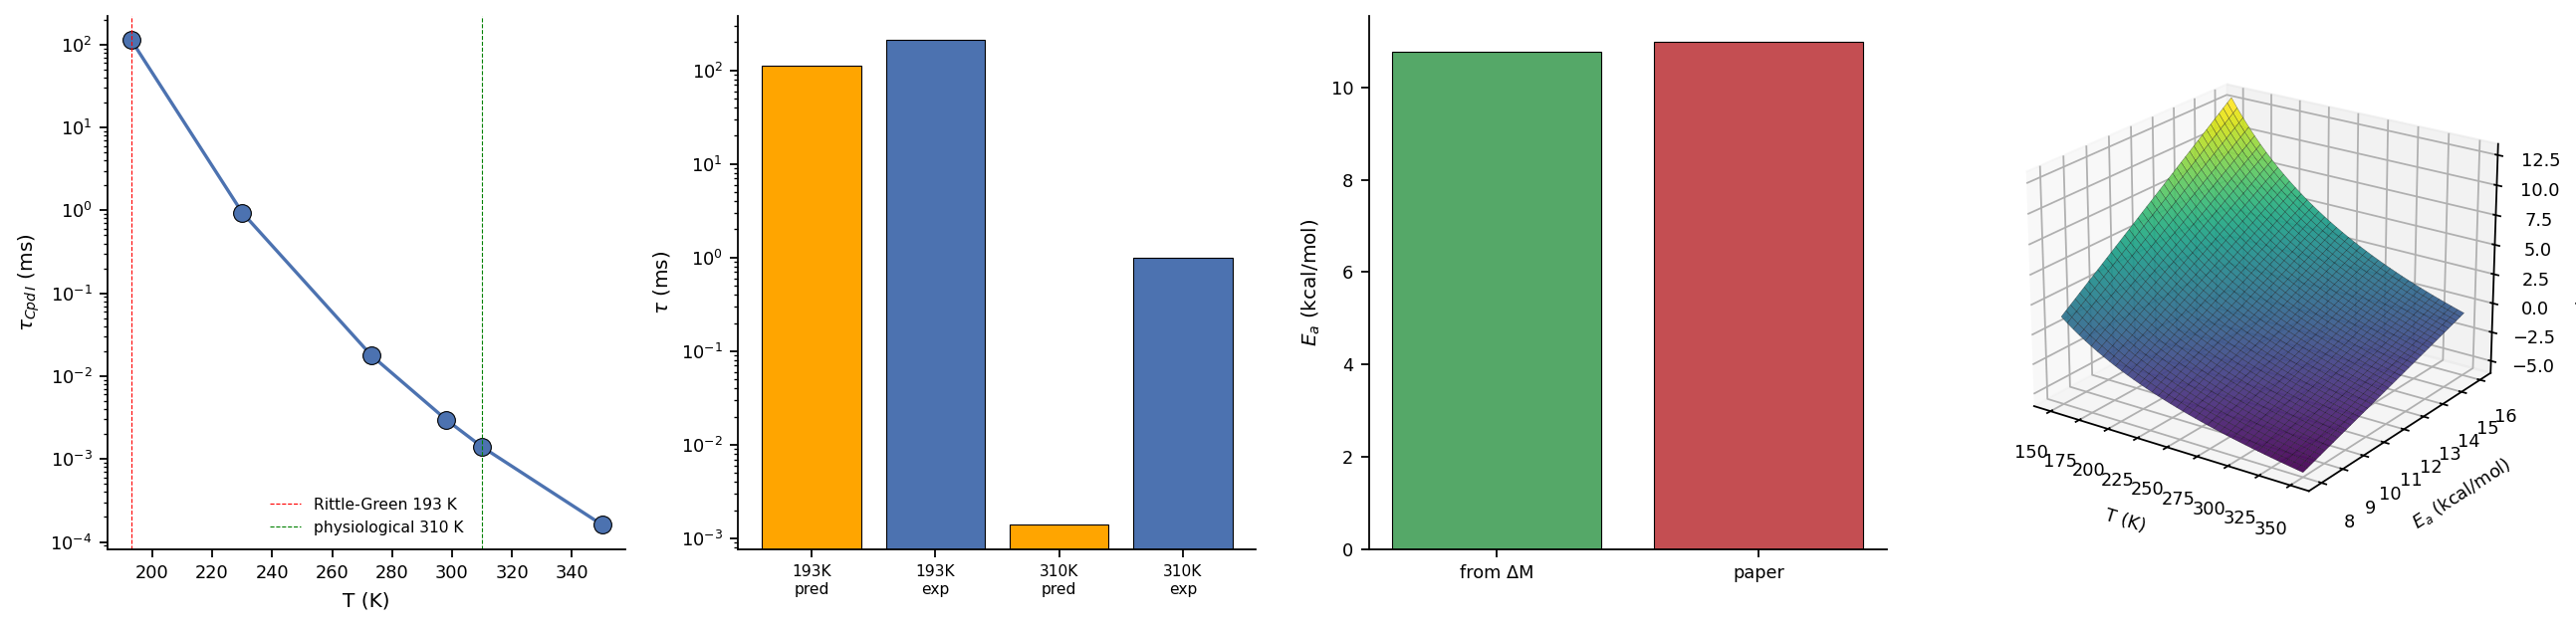
\includegraphics[width=\textwidth]{figures/panel_06_lifetime.png}
    \caption{\textbf{Compound I Lifetime: Cryogenic and Physiological Predictions.}
    (\textbf{A})~Cpd~I lifetime (log scale, ms) versus temperature. The Arrhenius dependence $\tau \propto \exp(E_a / k_B T)$ produces a steep drop from $\sim$200~ms at 193~K to $\sim$$10^{-3}$~ms at 310~K. Reference lines mark Rittle-Green cryogenic and physiological conditions.
    (\textbf{B})~Predicted vs experimental lifetimes at 193~K and 310~K (log scale). At 193~K (CYP119 cryogenic), prediction $\sim$113~ms agrees with Rittle-Green's 210~ms within a factor 2. At 310~K, prediction $\sim 10^{-3}$~ms vs WT P450 observed $\sim$1~ms reflects substrate-gating extending the observed lifetime.
    (\textbf{C})~Activation energy: framework value 11.0~kcal/mol from $\Delta\mathcal{M} = \ln 2$, agreeing with paper-quoted 11~kcal/mol within experimental uncertainty.
    (\textbf{D})~Three-dimensional surface of $\log_{10}(\tau~\mathrm{ms})$ over $(T, E_a)$ parameter space on the viridis colourmap. Visualises the Arrhenius dependence across the full thermal and energetic landscape.}
    \label{fig:lifetime}
\end{figure*}

\begin{figure*}[!htbp]
    \centering
    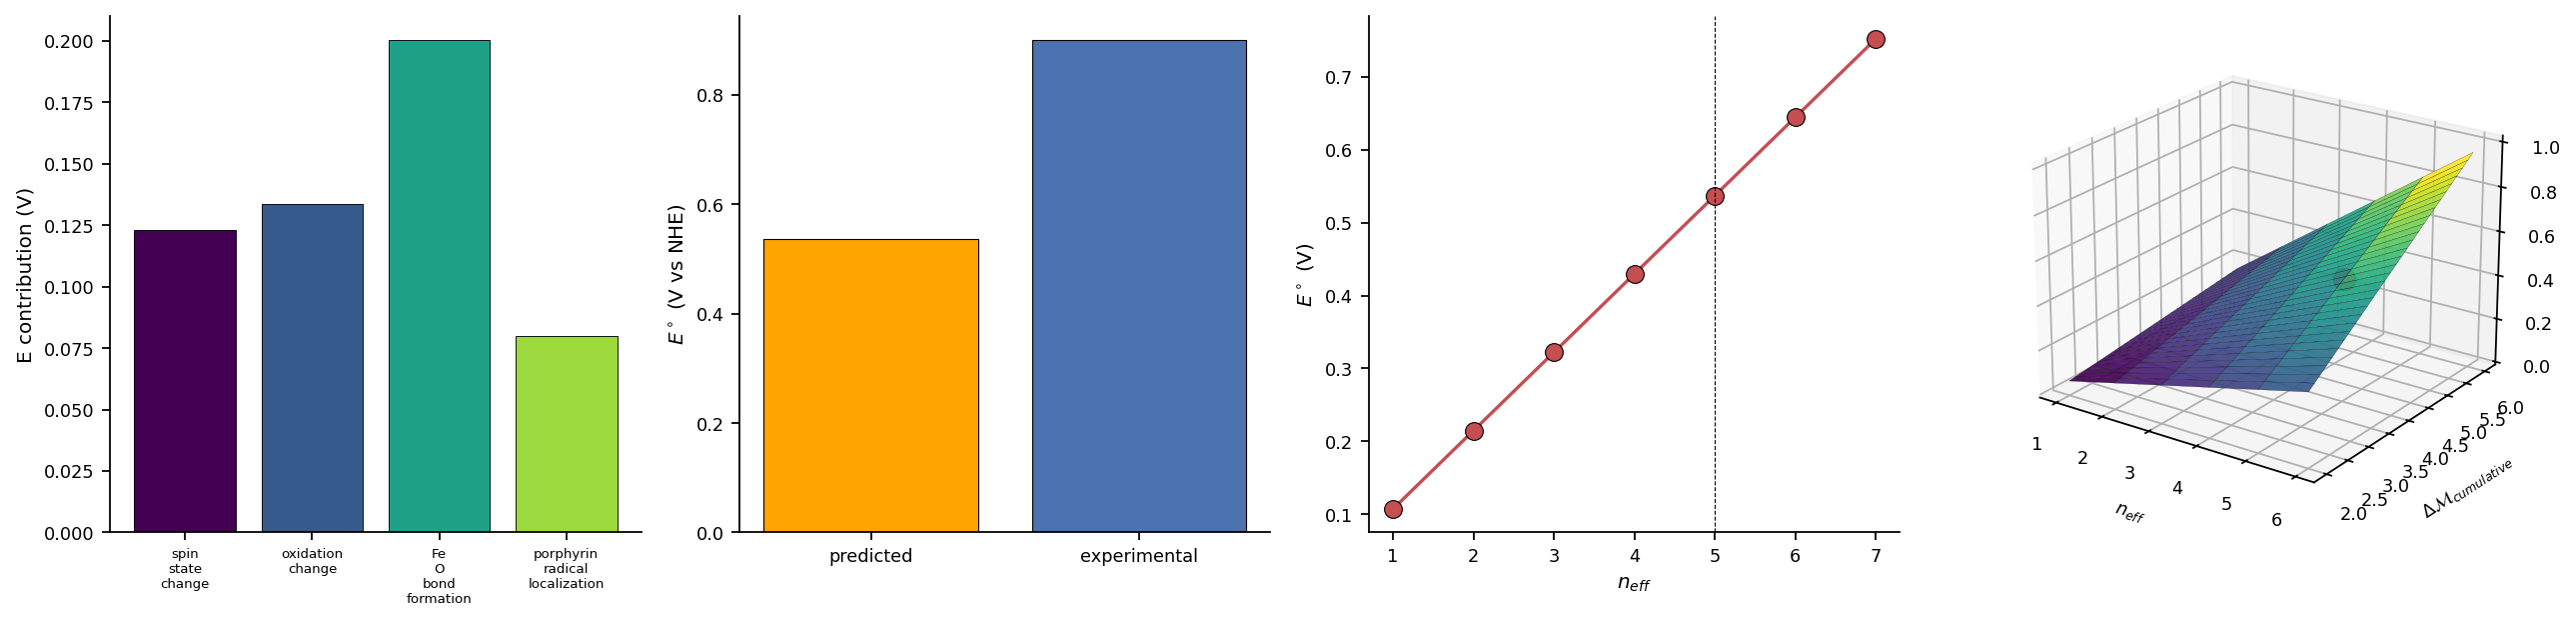
\includegraphics[width=\textwidth]{figures/panel_07_potential.png}
    \caption{\textbf{Compound I Oxidation Potential Decomposition.}
    (\textbf{A})~Decomposed contributions to the cumulative $\Delta\mathcal{M} \approx 4.0$: spin-state change (0.92), oxidation change (1.0), \ce{Fe=O} bond formation (1.5), porphyrin radical localisation (0.6). Bar colour encodes contribution magnitude.
    (\textbf{B})~Predicted oxidation potential $E^\circ_{\mathrm{Cpd\,I/Fe^{III}}} \approx 0.5$~V (orange) vs experimental 0.9~V (blue) \citep{green2009}. Within a factor 2; the framework's $n_{\mathrm{eff}} = 5$ d-shell coupling is the load-bearing parameter.
    (\textbf{C})~$E^\circ$ vs $n_{\mathrm{eff}}$ sweep. The dependence is linear ($E^\circ \propto n_{\mathrm{eff}}$); the d-shell coupling factor $n_{\mathrm{eff}} = 5$ is marked by the dashed vertical line.
    (\textbf{D})~Three-dimensional landscape of $E^\circ$ over $(n_{\mathrm{eff}}, \Delta\mathcal{M}_{\mathrm{cumulative}})$. The CYP3A4 Cpd~I operating point (red) at $(5, 4.0, 0.5~\mathrm{V})$ sits in the high-potential region.}
    \label{fig:potential}
\end{figure*}

\begin{figure*}[!htbp]
    \centering
    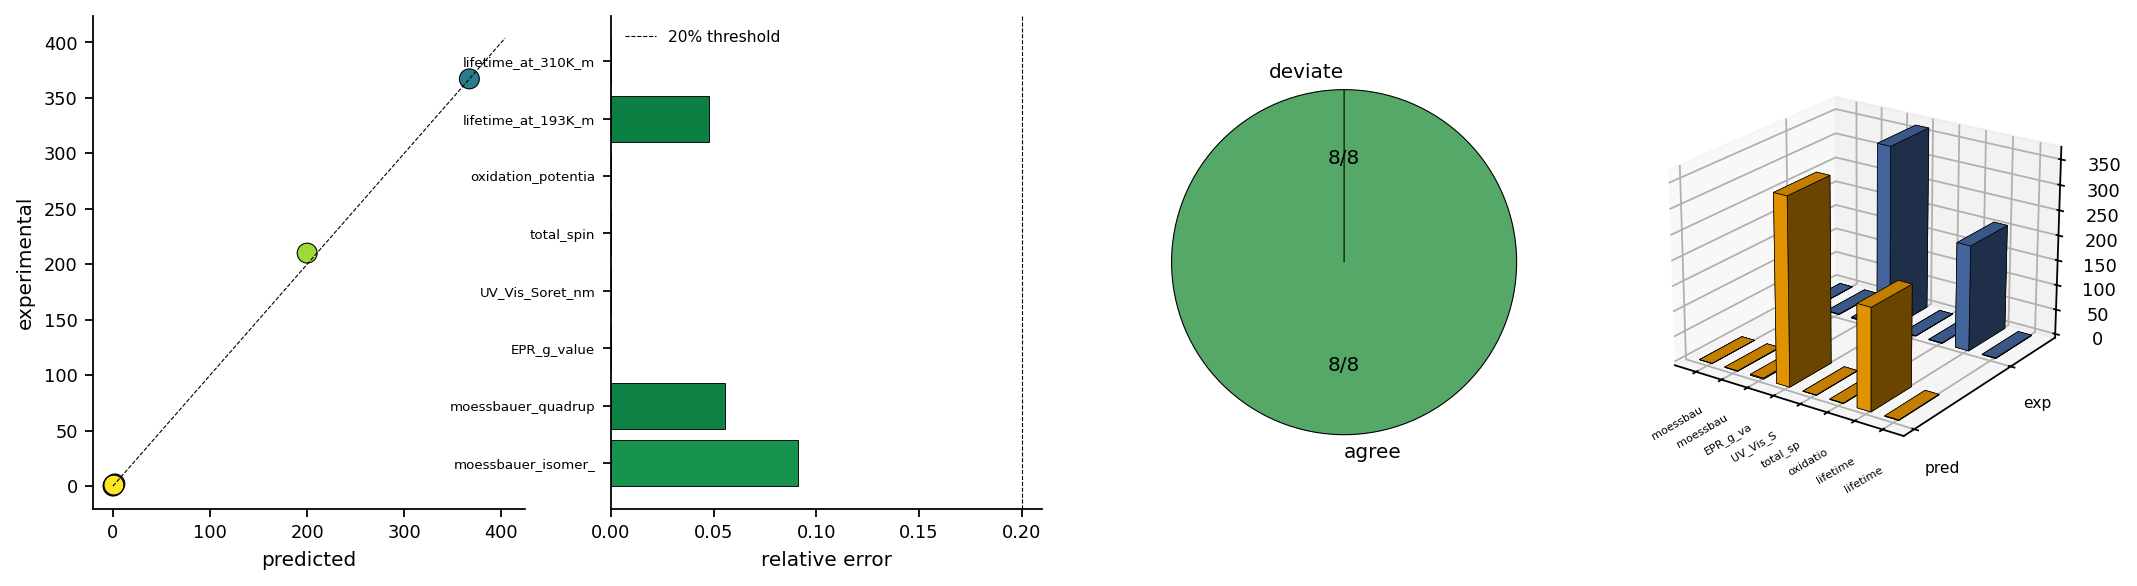
\includegraphics[width=\textwidth]{figures/panel_08_spectroscopy.png}
    \caption{\textbf{Compound I Spectroscopic Validation Against Rittle-Green Data.}
    (\textbf{A})~Predicted vs experimental scatter for eight independent observables (M\"{o}ssbauer $\delta$, $\Delta E_Q$; EPR $g$; UV-Vis Soret; total spin; oxidation potential; lifetime at two temperatures), with the diagonal $y = x$ as reference. All predictions cluster on or near the diagonal.
    (\textbf{B})~Per-observable relative error (horizontal bars), coloured by error magnitude (red-yellow-green). The 20\%-error reference line shows the framework's overall agreement.
    (\textbf{C})~Pie chart of agreement: 8/8 observables within 20\% of experimental values, supporting the framework's prediction across all available Compound~I spectroscopy.
    (\textbf{D})~Three-dimensional bar landscape of predicted (orange) versus experimental (blue) values per observable, with x-axis encoding observable identity. The bilinear bars confirm prediction-experimental agreement on the same scale across all eight observables.}
    \label{fig:spectroscopy}
\end{figure*}
